\documentclass{article}

\usepackage{amsmath,amssymb,amsthm}

\usepackage{hyperref}
\usepackage{graphicx}
\graphicspath{ {./img/} }

\usepackage{biblatex}
\addbibresource[
    style=authoryear
]{resources.bib}

\newtheorem{thm}{Theorem}
\newtheorem{def}{Definition}
\newtheorem{lem}{Lemma}
\newtheorem{proof}{Proof}
\newtheorem{rk}{Remark}
\newtheorem{cor}{Corollary}
\newtheorem*{lemm*}{Lemma}
\newtheorem*{variants}{}
\newtheorem*{var}{}

\renewcommand{\Rn}[1][n]{\mathbb{R}^{#1}}
\newcommand{\Absbars}[1]{\left\lVert#1\right\rVert}
\newcommand{\rmfd}[1]{Riemannian manifold}
\newcommand{\angle}[1]{\langle #1 \rangle}
\newcommand{\OM}{\Omega(M)}
\newcommand{\ome}{ $\omega$ }

\title{Ch. 12: The Energy of a Path}
\author{Nicolas Trutmann}
\date{}

\begin{document}


\includegraphics{img/qr.png}

link: \href{https://trn000.github.io/geodesics-seminar-talk/geodesics}{https://trn000.github.io/geodesics-seminar-talk/geodesics}

repo: \href{https://github.com/TrN000/geodesics-seminar-talk}{https://github.com/TrN000/geodesics-seminar-talk}


\maketitle





\subsection{Definitions and Motivation}

We'll prove what would seem intuitive, namely that geodesics are extrema of both length and energy of
a path between 2 points. That is the project we're working towards.

That was the point of geodesics in the first place when Gauss first introduced
them. They were defined with the intent of making a 'minimal path' between two
points; an analogue of the straight line in $\Rn$.


Let's first give the central definition of this chapter:

\begin{def}[Energy of a Path]
Let $\omega : \Rn[] \rightarrow M $ be a path on a \rmfd, with $\omega(a) = p$ and $\omega(b) = q$.
I.e. $\omega \in \Omega_{p,q}(M)$
\[ E_a^b(\omega) = \int_a^b \Absbars{\frac{d\omega}{dt}}^2 dt \]
\end{def}

This definition is styled after the similar kinetic energy equation
$\frac{1}{2}mv^2$.  Some authors even put $\frac{1}{2}$ in front of it to make
it look more like it. (We'll also see a factor 1/2 again.)

Compare this to the arc length functional from earlier in the book:

\[
     L_a^b(\omega) = \int_a^b \Absbars{\frac{d\omega}{dt}} dt
\]

If we apply Schwarz's inequality

\[
    \left( \int_a^b fg dt \right)^2
    \leq
    \left( \int_a^b f^2 dt \right)    \left( \int_a^b g^2 dt \right)
\]

with $f = 1$ and $g = \Absbars{\frac{d\omega}{dt}}$ we see that

\[
    \left( L_a^b \right)^2
    \leq
    (b - a)\left( E_a^b \right)
\]

with equality iff the function $g$ is constant, that is the parameter $t$ is
proportional to arc length.

\begin{lem}
    \label{lem:geod-min}
    Let $M$ be a complete \rmfd and let $p,q \in M$ have distance $d$. Then the energy function
    \[
        E: \Omega(M;p,q) \rightarrow R
    \]
    takes on its minimum precisely on the set of minimal geodesics from $p$ to $q$.
\end{lem}


\begin{proof}
    Suppose that there exists a minimal geodesic $\gamma$ from $p = \omega(0)$
    to $q = \omega ( 1 )$. Then
    \[E(\gamma) = L(\gamma)^2 \leq L( \omega )^2 \leq E(w) \]
    Here the equality $L( \gamma ) = L(\omega)$ can hold only if $\omega$ is also a minimal
    geodesic, possibly reparametrized.
    On the other hand the equality $L ( \omega )^2 = E( \omega)$ can hold only if the parameter is proportional
    to arc length along $\omega$ . This proves that $E ( \omega ) < E(\omega)$ unless $\omega$ is also
    a minimal geodesic.
\end{proof}







\subsection{The proportional-to-arc-length argument}

A problem with curves is that we could parametrize them arbitrarily badly.

The concept of a geodesic in a manifold generalizes that of a straight line in
Euclidean space. A straight line in $\Rn[2]$ has parametrizations of form $t
\mapsto \gamma → p + \sigma(t)v$ where $\sigma : \Rn[] → \Rn[]$ is a
diffeomorphism and $p, v \in \Rn[]$.

Different choices of $\sigma$ yield different parametrizations of the same
line. Certain parametrizations are preferred, for example those
parametrizations which are "proportional to the arc length", i.e. where
$\sigma(t) = at + b$ for constants $a, b \in \Rn[]$, so that the tangent vector
$\dot{\sigma}(t)v$ has constant length.

Arc length is invariant under reparametrization but energy need not be.

\begin{rk}[Reparametrization]
    Let $I = [a, b]$ and $I' = [a', b']$ be compact intervals. If $\gamma : I
    \rightarrow \Rn$ is a smooth curve and $\sigma : I' \rightarrow I$ is a
    smooth function such that $\sigma(a') = a$, $\sigma(b') = b$, and
    $\dot{\sigma}(t') ≥ 0$ for all $t' \in I'$, then the curves $\gamma$ and
    $\gamma \circ \sigma$ have the same length. Namely,
    \[
        L(\gamma  \circ \sigma)
        = \int_{a'}^{b'} \left|\frac{d}{dt} \gamma(\sigma(t')) \right| dt'
        = \int_{a'}^{b'} \left|\frac{d}{dt} \dot{\gamma}(\sigma(t')) \right| \dot{\sigma}(t') dt'
        = L(\gamma  \circ \sigma)
        \
    \]
    Here second equality follows from the chain rule and the third equality
    follows from the change of variables formula for the Riemann integral.
\end{rk}




\subsection{sleight of hand: calculus of variations}

The big cheat of these chapters is that we're able to do calculus on $\OM$.
This is a priori not a manifold, topological space, vector field or group.
It becomes, however, after doing some math to it.

In Milnor's book \cite{milnor}, this problem is explicitly brushed under the table.
Books that treat the matter more thoroughly brush it under the table with a few more words
\cite{salamon} 4.1.7.
Here is a reference that is explicit and thorough: \cite{lee}

Since Milnor hand-waves the problem, so will we. Since we still need intuition for what we're
skipping I provide here two pictures, which we will pretend is how all the curves under scrutiny
look like.

\begin{figure}
    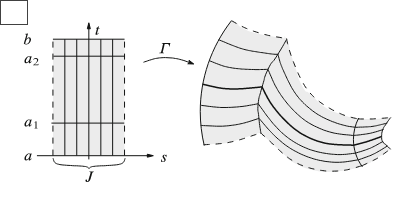
\includegraphics{img/grid.png}
    \caption{grid shape}
    \label{fig:grid}
\end{figure}
\begin{figure}
    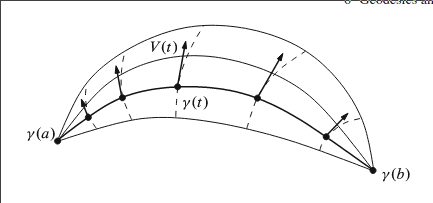
\includegraphics{img/sail.png}
    \caption{variation of a curve}
    \label{fig:sail}
\end{figure}



What we'll need in particular is the vector field along a variation.

Reminder:

\begin{def}
\label{def:vel_of_var}
    The velocity of a variation $\alpha: (-\epsilon, \epsilon) \rightarrow \Omega(M;p,q)$ with
    $\alpha(0) = \omega$ is defined as

    \[ W_t = \frac{d\alpha}{du}(0)_t = \frac{d\alpha}{du}(0, t) \]

    It is the \textbf{variation vector field} $W \in T\Omega_{\omega}$.
\end{def}
\subsection{Theorem 12.1}


Recall:
\[
    \begin{align*}
        W_t &= \frac{d\alpha}{du} \quad\text{derivative of the variation} \\
        V_t &= \frac{d\omega}{dt} \quad\text{velocity of $\omega$} \\
        \Delta_tV &= V_{t+} - V_{t-} \quad\text{discontinuity in the velocity vector} \\
        A_t &= \frac{D}{dt} \frac{d\omega}{dt} \quad\text{acceleration of $\omega$} \\
    \end{align*}
\]

$\Delta_tV = 0$ for all but finitely many points.


\begin{thm}[Milnor's 12.1]
    \label{thm:12.1}

    For a variation $\alpha$ of $\omega$, we have:

    \[
        \frac{1}{2} \frac{dE(\alpha(u))}{du} =
        \sum_{k} \angle{ W_t, \Delta_tV } \ \ + \ \ \int_0^1 \angle{ W_t, A_t }
    \]

\end{thm}

As a reminder without proof, a lemma from the book.

\begin{lemm*}[Lemma 8.3]
    For a compatible connection (read: Levi-Civita) and any vector fields $V,W$ along a curve
    $\gamma$, we have
    \[
        \frac{d}{dt}\langle V, W \rangle   =
        - \langle \frac{DV}{dt}, W \rangle - \langle V, \frac{DW}{dt} \rangle
    \]
\end{lemm*}



\begin{proof}[proof of \ref{thm:12.1}]
    To begin the proof let's talk about the intuition of what we're writing down here.

    What we care about in this equation is not the equation itself, but when it is zero. We are
    searching for extremal points of our variation.

    The first part of the equation tells us what we can expect from "kinks" in our curve. They will
    add to the derivative, which suggests that kink-free or smooth curves are candidates for
    geodesics.

    The second part concerns the acceleration must be orthogonal to $W_t$ to be identically zero.
    The intuitive interpretation is that our curve may not curve.

    Together with the fact that the velocity $V_t$ is constant it follows that the acceleration is
    normal on the tangent space.


    \begin{figure}
        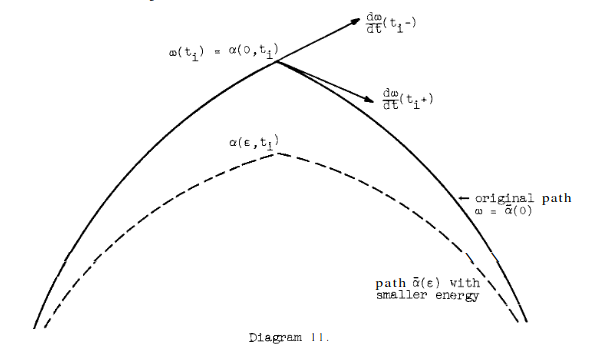
\includegraphics{img/kinky.png}
        \caption{kinks in our curves}
        \label{fig:kinky}
    \end{figure}


    The proof itself follows from a very direct computation.


    Take the left-hand side and insert definitions.

    \[
        \frac{1}{2} \frac{dE(\alpha(u))}{du} =
        \frac{d}{du} \int_0^1 \angle{\frac{\partial \alpha}{\partial t}, \frac{\partial \alpha}{\partial t}} =
        2 \int_0^1 \angle{\frac{D}{du} \frac{\partial \alpha}{\partial t}, \frac{\partial \alpha}{\partial t}}
    \]

    By Lemma 8.5 we can substitute
    $\frac{D}{dt} \frac{\partial \alpha}{\partial u}$ for
    $\frac{D}{du} \frac{\partial \alpha}{\partial t}$ in this last formula.

    Next, we partition $t$ at the discontinuous parts into $0 \lt t_1 \lt \ldots \lt t_k \lt 1$,
    such that $\alpha$ is differentiable on the intervals $[t_i, t_{i+1}]$.

    On these intervals we do "integration by parts" of sorts, by using the identity

    \[
        \frac{d}{dt} \angle{\frac{\partial \alpha}{\partial u}, \frac{\partial \alpha}{\partial t}} =
        \angle{\frac{D}{\partial t} \frac{\partial \alpha}{\partial u}, \frac{\partial \alpha}{\partial t}}
        +
        \angle{\frac{\partial \alpha}{\partial t}, \frac{D}{\partial t} \frac{\partial \alpha}{\partial t}}
    \]

    this implies

    \[
        \int_{t_{i-1}}^{t_i} \angle{\frac{D}{\partial t} \frac{\partial \alpha}{\partial u}, \frac{\partial \alpha}{\partial t}}
        =
        \left.  \angle{\frac{\partial \alpha}{\partial u}, \frac{\partial \alpha}{\partial t}} \right\vert_{t=t_{i-1} +}^{t=t_i -}
        -
        \int_{t_{i-1}}^{t_i} \angle{\frac{\partial \alpha}{\partial t}, \frac{D}{\partial t} \frac{\partial \alpha}{\partial t}}
    \]

    Gluing these together yields the desired formula. The first term works like
    an inverse telescoping sum, where the inner terms don't cancel out and the
    first and last terms disappear, since $\partial \alpha / \partial u = 0$ at
    the end points.

    \[
        \frac{1}{2} \frac{dE(\alpha(u))}{du}
        =
        - \sum_{i=1}^{k-1} \angle{\frac{\partial \alpha}{\partial u}, \Delta \frac{\partial \alpha}{\partial t}}
        -
        \int_{0}^{1} \angle{\frac{\partial \alpha}{\partial t}, \frac{D}{\partial t} \frac{\partial \alpha}{\partial t}}
    \]

    And at $u = 0$

    \[
        \frac{1}{2} \frac{dE(\alpha(u))}{du}
        =
        - \langle \frac{DV}{dt}, W \rangle - \langle V, \frac{DW}{dt} \rangle
    \]

    unfinished
\end{proof}

\begin{cor}
    The path $\omega$ is a critical point for the function $E$ if and only if $\omega$ is a geodesic.
\end{cor}

\begin{proof}

    "$\Leftarrow$": From the earlier Lemma \ref{lem:geod-min} we know that the energy function takes on its minimum on geodesics so it follows that it is a critical point.

    "$\Rightarrow$":


    Let \ome be a critical point . There is a variation of \ome with $W(t) = f (t)A(t)$ where
    $f(t)$ is positive.
    Then
    \[
        \frac{1}{2}\frac{dE}{du} = - \int_0^1 f(t) \angle{A(t), A(t)} dt
    \]
    This is zero if and only if $A(t) = 0$ for all $t$.

    Now we treat the discontinuities. At the $t_i$ where \ome is discontinuous we have
    $\frac{1}{2}\frac{dE}{du} = -\sum \angle{\Delta_{t_i}V, \Delta_{t_i}V}$ which can only be zero when all $\Delta_{t_i}V$ are zero.


\end{proof}



\subsection{Recap: Characterization Theorem}


I grabbed this theorem from another book (\cite{salamon} 4.1.4).
We have done about the same work, just in a different order.
It works as a nice summary of the discussed material.

\begin{thm}[Characterization of Geodesics]
    Let $I = [a, b] \subset \Rn[]$ be a compact interval and let $\omega : I \rightarrow M$ be a
    smooth curve. Then the following are equivalent.

    \begin{enumerate}
        \item
            (definition)
            The velocity vector of $\omega$ is parallel, i.e. $\nabla  ̇\omega(t) = 0$ for all $t \in I$.
        \item
            (extremal energy) $\omega$ is an extremal of the energy functional, i.e. every variation $\alpha \in \Omega(M)$
            of $\omega$ with fixed endpoints satisfies
            \[
                \frac{d}{dt} E(\omega) = 0
            \]
        \item
            (extremal length)
            $\omega$ is parametrized proportional to the arc length, i.e. the velocity
            $\dot{\omega}(t) \equiv c ≥ 0$ is constant, and either $\omega$ is constant, i.e. $\omega(t) = p = q$ for
            all $t \in I$, or $c > 0$ and $\omega$ is an extremal of the length functional, i.e.
            every variation $\alpha \in \Omega(M)$ of $\omega$ with fixed endpoints satisfies
            \[
                \frac{d}{dt} L(\omega) = 0
            \]
        \item
            (perpendicular acceleration)
            The acceleration of $\omega$ is normal to $M$ , i.e. $\ddot{\omega}(t) \perp T_{\omega(t)}M$ for all $t \in I$.
    \end{enumerate}
\end{thm}


\begin{proof}
    \cite{salamon} 4.1.3
\end{proof}


\subsection{Bibliography}

\printbibliography

\end{document}
